\documentclass[
	% -- opções da classe memoir --
	12pt,				% tamanho da fonte
	openright,			% capítulos começam em pág ímpar (insere página vazia caso preciso)
	oneside,			% para impressão em verso e anverso. Oposto a oneside
	a4paper,			% tamanho do papel. 
	% -- opções da classe abntex2 --
	%chapter=TITLE,		% títulos de capítulos convertidos em letras maiúsculas
	%section=TITLE,		% títulos de seções convertidos em letras maiúsculas
	%subsection=TITLE,	% títulos de subseções convertidos em letras maiúsculas
	%subsubsection=TITLE,% títulos de subsubseções convertidos em letras maiúsculas
	% -- opções do pacote babel --
	english,			% idioma adicional para hifenização
	french,				% idioma adicional para hifenização
	spanish,			% idioma adicional para hifenização
	brazil,				% o último idioma é o principal do documento
	]{abntex2}


% ---
% PACOTES
% ---
% ---
% Pacotes fundamentais 
% ---
\usepackage{cmap}				% Mapear caracteres especiais no PDF
%\usepackage{lmodern}			% Usa a fonte Latin Modern		
\usepackage{helvet}
\usepackage[T1]{fontenc}		% Selecao de codigos de fonte.
\usepackage[utf8]{inputenc}		% Codificacao do documento (conversão automática dos acentos)
\usepackage{lastpage}			% Usado pela Ficha catalográfica
\usepackage{indentfirst}		% Indenta o primeiro parágrafo de cada seção.
\usepackage{color}				% Controle das cores
\usepackage{graphicx}			% Inclusão de gráficos
\usepackage{underscore}
\usepackage{amsfonts}
\usepackage{listings}
% ---
\linespread{1.5} % espaçamento entre linhas		
% ---
% Pacotes adicionais, usados apenas no âmbito do Modelo Canônico do abnteX2
% ---
\usepackage{lipsum}				% para geração de dummy text
\usepackage{amsmath}
% ---

% ---
% Pacotes de citações
% ---
\usepackage[brazilian,hyperpageref]{backref}	 % Paginas com as citações na bibl
\usepackage[alf]{abntex2cite}	% Citações padrão ABNT
\usepackage{longtable}
\usepackage{hyperref}
\hypersetup{
    colorlinks=false,
    pdfpagemode=FullScreen,
    pdftitle={benchmark bancos de dados multi arquitetura},
}
\hypersetup{final}
\urlstyle{same}
% --- 
% CONFIGURAÇÕES DE PACOTES
% --- 

% ---
% Configurações do pacote backref
% Usado sem a opção hyperpageref de backref
%\renewcommand{\backrefpagesname}{Citado na(s) página(s):~}
\renewcommand{\backrefpagesname}{}
% Texto padrão antes do número das páginas
\renewcommand{\backref}{}
% Define os textos da citação
\renewcommand*{\backrefalt}[4]{
	\ifcase #1 %
		Nenhuma citação no texto.%
	\or
		%Citado na página #2.%
	\else
		%Citado #1 vezes nas páginas #2.%
	\fi}%
% ---


% ---
% Informações de dados para CAPA e FOLHA DE ROSTO
% 
\titulo{Benchmark de desempenho entre bancos de dados em diferentes arquiteturas}

\autor{Miguel Magalhães Lopes}
\local{Rio Pomba}
\data{20XX}
\orientador{Gustavo Henrique da Rocha Reis}
\coorientador{CICLANO}
%\instituicao{}
\tipotrabalho{Trabalho de Conclusão de Curso}
% O preambulo deve conter o tipo do trabalho, o objetivo, 
% o nome da instituição e a área de concentração 
\preambulo{Trabalho de Conclusão apresentado ao Campus Rio Pomba, do Instituto Federal de Educação, Ciência e Tecnologia do Sudeste de Minas Gerais, como parte das exigências do curso de Bacharelado em Ciência da Computação para a obtenção do título de Bacharel em Ciência da Computação.}
% ---


% ---
% Configurações de aparência do PDF final

% alterando o aspecto da cor azul
\definecolor{blue}{RGB}{41,5,195}

% informações do PDF
%\makeatletter
%\hypersetup{
     	%pagebackref=true,
%		pdftitle={\@title}, 
%		pdfauthor={\@author},
%    	pdfsubject={\imprimirpreambulo},
%	    pdfcreator={Matheus F O Baffa},
%		pdfkeywords={content-based image retrieval}{desenvolvimento web}{exame de fundo de olho}{histograma backprojection}{íris}, 
%		colorlinks=true,       		% false: boxed links; true: colored links
%    	linkcolor=black,          	% color of internal links
%    	citecolor=black,        		% color of links to bibliography
%    	filecolor=black,      		% color of file links
%		urlcolor=black,
%		bookmarksdepth=4
%}
\makeatother
\graphicspath{ {./imagens/} }
% --- 

% --- 
% Espaçamentos entre linhas e parágrafos 
% --- 

% O tamanho do parágrafo é dado por:
\setlength{\parindent}{1.3cm}

% Controle do espaçamento entre um parágrafo e outro:
\setlength{\parskip}{0.2cm}  % tente também \onelineskip

% ---
% compila o indice
% ---
\makeindex
% ---

% ----
% Início do documento
% ----
\begin{document}

% Retira espaço extra obsoleto entre as frases.
\frenchspacing 

% ----------------------------------------------------------
% ELEMENTOS PRÉ-TEXTUAIS
% ----------------------------------------------------------
% \pretextual

% ---
% Capa
% ---
\begin{center}
\textbf{ 
INSTITUTO FEDERAL DE EDUCAÇÃO, CIÊNCIA E TECNOLOGIA DO SUDESTE DE MINAS GERAIS - CAMPUS RIO POMBA}
\end{center}

\imprimircapa
% ---

% ---
% Folha de rosto
% (o * indica que haverá a ficha bibliográfica)
% ---
\imprimirfolhaderosto*
% ---

% ---
% Inserir a ficha bibliografica
% ---

% Isto é um exemplo de Ficha Catalográfica, ou ``Dados internacionais de
% catalogação-na-publicação''. Você pode utilizar este modelo como referência. 
% Porém, provavelmente a biblioteca da sua universidade lhe fornecerá um PDF
% com a ficha catalográfica definitiva após a defesa do trabalho. Quando estiver
% com o documento, salve-o como PDF no diretório do seu projeto e substitua todo
% o conteúdo de implementação deste arquivo pelo comando abaixo:
%
% \begin{fichacatalografica}
%     \includepdf{fig_ficha_catalografica.pdf}
% \end{fichacatalografica}
\begin{fichacatalografica}
	\vspace*{\fill}					% Posição vertical
	\hrule							% Linha horizontal
	\begin{center}					% Minipage Centralizado
	\begin{minipage}[c]{12.5cm}		% Largura
	
	\imprimirautor
	
	\hspace{0.5cm} \imprimirtitulo  / \imprimirautor. --
	\imprimirlocal, \imprimirdata-
	
	\hspace{0.5cm} \pageref{LastPage} p. : il. (algumas color.) ; 30 cm.\\
	
	\hspace{0.5cm} \imprimirorientadorRotulo~\imprimirorientador\\
	
	\hspace{0.5cm}
	\parbox[t]{\textwidth}{\imprimirtipotrabalho~--~Instituto Federal de Educação, Ciência e Tecnologia do Sudeste de Minas, Campus Rio Pomba,
	\imprimirdata.}\\
	
	\hspace{0.5cm}
		1. 
		2. 
		I. 
		II.
		III.
		IV. \\ 			
	
	\hspace{8.75cm} %CDU 02:141:005.7\\
	
	\end{minipage}
	\end{center}
	\hrule
\end{fichacatalografica}
% ---

% ---
% Inserir errata
% ---
%\begin{errata}
%Elemento opcional da \citeonline[4.2.1.2]{NBR14724:2011}. %Exemplo:

%\vspace{\onelineskip}
%
%FERRIGNO, C. R. A. \textbf{Tratamento de neoplasias ósseas apendiculares com
%reimplantação de enxerto ósseo autólogo autoclavado associado ao plasma
%rico em plaquetas}: estudo crítico na cirurgia de preservação de membro em
%cães. 2011. 128 f. Tese (Livre-Docência) - Faculdade de Medicina Veterinária e
%Zootecnia, Universidade de São Paulo, São Paulo, 2011.

%\begin{table}[htb]
%\center
%\footnotesize
%\begin{tabular}{|p{1.4cm}|p{1cm}|p{3cm}|p{3cm}|}
%  \hline
%   \textbf{Folha} & \textbf{Linha}  & \textbf{Onde se lê} % & \textbf{Leia-se}  \\
%    \hline
%    1 & 10 & auto-conclavo & autoconclavo\\
%   \hline
%\end{tabular}
%\end{table}
%
%\end{errata}
% ---

% ---
% Inserir folha de aprovação
% ---

% Isto é um exemplo de Folha de aprovação, elemento obrigatório da NBR
% 14724/2011 (seção 4.2.1.3). Você pode utilizar este modelo até a aprovação
% do trabalho. Após isso, substitua todo o conteúdo deste arquivo por uma
% imagem da página assinada pela banca com o comando abaixo:
%
% \includepdf{folhadeaprovacao_final.pdf}
%
\begin{folhadeaprovacao}

  \begin{center}
    {\ABNTEXchapterfont\large\imprimirautor}

    \vspace*{\fill}\vspace*{\fill}
    {\ABNTEXchapterfont\bfseries\Large\imprimirtitulo}
    \vspace*{\fill}
    
    \hspace{.45\textwidth}
    \begin{minipage}{.5\textwidth}
        \imprimirpreambulo
    \end{minipage}%
    \vspace*{\fill}
   \end{center}
    
   Trabalho aprovado. \imprimirlocal, 00 de dezembro de 20XX.

   \assinatura{\textbf{\imprimirorientador}, Orientador, IF Sudeste MG - Rio Pomba} 
   \assinatura{\textbf{CICLANO}, Coorientador, IF Sudeste MG - Rio Pomba}
   \assinatura{\textbf{Dr. BELTRANO} \\ IF Sudeste MG - Rio Pomba}
   \assinatura{\textbf{Me. XXXXXXXXXXXXX} \\ IF Sudeste MG - Rio Pomba }
   %\assinatura{\textbf{Professor W} \\ IF Sudeste MG - Rio Pomba}
      
   \begin{center}
    \vspace*{0.5cm}
    {\large\imprimirlocal}
    \par
    {\large\imprimirdata}
    \vspace*{1cm}
  \end{center}
  
\end{folhadeaprovacao}
% ---


% ---
% Dedicatória
% ---
\begin{dedicatoria}
   \vspace*{\fill}
	\begin{flushright}
        Este trabalho é dedicado a todos\\ 
       aqueles que me inspiraram, em especial\\ 
       XXXXXXXXXXXXXXXXXXXXXXXXXXXXXXXXX \\
       XXXXXXXXXXXXXXXXXXXXXXXXXXXXXXXXXXXXXXXXXX.
    \end{flushright}
\end{dedicatoria}
% ---

% ---
% Agradecimentos
% ---
\begin{agradecimentos}

\end{agradecimentos}

% resumo em português
\begin{resumo}
\noindent

 \vspace{\onelineskip}
    
 \noindent
 \textbf{Palavras-chaves:} palavra1. palavra2. palavra3. palavra4.
\end{resumo}

% resumo em inglês
\begin{resumo}[Abstract]
 \begin{otherlanguage*}{english}
   \vspace{\onelineskip}
    \noindent 

   \vspace{\onelineskip}
   
   \noindent  \textbf{Key-words}:  word1. word2. word3. word4. word5.
 \end{otherlanguage*}
\end{resumo}
\urlstyle{same}

\pdfbookmark[0]{\listfigurename}{lof}
\listoffigures*
\cleardoublepage

\pdfbookmark[0]{\listtablename}{lot}
\listoftables*
\cleardoublepage

\DeclareRobustCommand{\beginAutoTable}[4]{
%nome da tabela e label
%cabeçalho
%quantidade total de colunas
%formatação da tabela
\label{tab:#1}
  \begin{longtable}{#4}
  \caption{#1}
\\ \hline \multicolumn{#3}{c}{\textbf{#1}} \\ \hline 
#2 \\ \hline \endfirsthead
#2 \\ \hline \endhead
}
\newenvironment{easyTableAuto}[4]{
\beginAutoTable{#1}{#2}{#3}{#4}
}{
  \end{longtable}
}
\newenvironment{easyTable2}[2]{
\beginAutoTable{#1}{#2}{2}{p{.15\textwidth}|p{.80\textwidth}}
}{
  \end{longtable}
}
\newenvironment{easyTable3}[2]{
\beginAutoTable{#1}{#2}{3}{p{.16\textwidth}|p{.1\textwidth}|p{.70\textwidth}}
}{
  \end{longtable}
}
\DeclareRobustCommand{\myref}[2]{
\textit{#2}$^{\text{#1\ref{#1:#2}}}$
}
\newcounter{sig}
\DeclareRobustCommand{\sig}[1]{
   \refstepcounter{sig}
   \label{sig:#1}
   \item[#1]
   }
\newcounter{ch}
\DeclareRobustCommand{\ch}[1]{
   \refstepcounter{ch}
   \chapter{#1}
   \label{ch:#1}
   }
\newcounter{sec}
\DeclareRobustCommand{\sec}[1]{
   \refstepcounter{sec}
   \section{#1}
   \label{sec:#1}
   }
\newcounter{subsec}
\DeclareRobustCommand{\subsec}[1]{
   \refstepcounter{subsec}
   \subsection{#1}
   \label{subsec:#1}
   }

\begin{siglas}
    \sig{DACC} Departamento Acadêmico de Ciência da Computação
    
    \sig{UFJF} Universidade Federal de Juiz de Fora
    
    \sig{arm} ARM, originalmente Acorn RISC Machine, e depois Advanced RISC Machine, é uma família de arquiteturas RISC desenvolvida pela empresa britânica ARM Holdings
    
    \sig{IDE} 
    
    \sig{x64}
    
    \sig{x86}
    
    \sig{aarch64}
    
    \sig{ram}
    
    \sig{GPU}
    
    \sig{TPU}
    
    \sig{CPU}
    
    \sig{JVM} JVM (Java Virtual Machine) é uma máquina abstrata. É uma especificação que fornece um ambiente de tempo de execução no qual o bytecode do java pode ser executado.
As JVMs estão disponíveis para muitas plataformas de hardware e software (ou seja, a JVM depende da plataforma).
    
    \sig{IOT}
    
    \sig{SBC}
    
    \sig{BIOS}
    
    \sig{TTL}
    
    \sig{UART}
    
    \sig{WINE}
    
\end{siglas}


\tableofcontents*

\textual
\setcounter{page}{1}
% ---------------------------------------------------------------------------------------------
% Introdução
% ---------------------------------------------------------------------------------------------
\chapter*{Introdução}
\addcontentsline{toc}{chapter}{\textbf{Introdução}}
\markright{Introdução}
\label{ch:introducao}
%\ch{introducao}
Esta pesquisa foi baseada na crescente adoção de processadores \myref{sig}{arm}, que conseguem entregar uma eficiência energética muito superior a comumente utilizada nos computadores e servidores (de arquitetura \myref{sig}{x86}).
Esta arquitetura possui uma versão 64 bit, que hoje em dia é praticamente a única variante utilizada a \myref{sig}{x64}. Essa arquitetura é, no geral,
apenas uma variante aditiva da \myref{sig}{x86} na qual são adicionadas varias instruções e vários suportes, sendo o principal deles o suporte a comandos 64 bits.
O mesmo pode ser dito para a arquitetura \myref{sig}{aarch64} ou arm64 que é uma variante aditiva da \myref{sig}{arm},essa não é ,como a \myref{sig}{x64} uma versão única,
mas sim uma "denominação" das variantes e evoluções da arquitetura \myref{sig}{arm} com suporte a 64bit.As arquiteturas passaram a ser denominadas dessa forma a partir da armv8,
entretanto existem versões do \myref{sig}{arm},como o armv7l, que consegue trabalhar com instruções de 64bit,apesar de ser uma arquitetura 32 bits.\newline
O foco da pesquisa foi feito em cima do uso de servidores \myref{sig}{arm}, que é baixo, apesar de totalmente possível e existente no mundo corporativo.
Existem alguns servidores comerciais que utilizam a arquitetura \myref{sig}{arm} para seu funcionamento. Desta forma foi feita uma comparação na utilização desses processadores para a simulação de uma aplicação de banco de dados. 
Essa aplicação simula a utilização de forma realística de uma base de dados de uma locadora. \newline
O cenário foi escolhido a partir de um esquema de banco de dados genérico da internet e foram utilizados os bancos de dados PostgreSQL e MariaDB, visto que são os bancos de dados de propósito geral mais utilizados atualmente.
Foi preferido o MariaDB sobre o MySQL visto que não existe uma versão dele para a arquitetura \myref{sig}{arm} e ambos são basicamente o mesmo sistema.\newline
Foi criado um programa para a geração de dados realísticos baseados na biblioteca faker implementada na linguagem Python. Estes dados são gerados para cada país específico em idiomas e caracteres compatíveis com a região escolhida.
Desta forma é plausível que estes dados, como nome, telefone, endereço e até mesmo usuário e senha sejam possíveis de existirem.
Foi escolhido essa forma de inserção pois um preenchimento de dados totalmente randômico e de tamanho fixo podem apresentar discrepâncias com o desempenho num ambiente real de uso,
afetando tanto o tempo, quanto carga dos processadores de forma negativa. Os dados utilizados em cada teste são exatamente os mesmos, com a diferença apenas da quantidade,
simbolizando o uso em um ambiente real. Desta fomra o benchmark se torna mais aplicável a realidade.\newline

%\chapter{Fundamentação Teórica}
%\label{ch:fundamentacao teorica}
\ch{fundamentacao teorica}

\sec{virtualização}
virtualização é uma tecnica usada para simular um computador dentro de outro,dependendo do método utilizado ele pode simular apenas uma camada ou mais de uma das camadas de hardware e software de um computador .
um computador virtualizado pode receber varios nomes dependendo do método utilizado para virtualizar,os mais utilizados hoje em dia são maquinas virtuais e containers docker,
a principal difetença deles é a camada de harware na qual ele executa

\sec{maquina virtual}
uma maquina virtual é rodada por um programa dentro de um sistema operacional,maquinas virtuais possuem varias limitações,
dentre elas por rodar em uma camada de software ele possui um menor desempenho de cpu e não pode ter acesso a outros hardwares do computador ,
na maioria dos mecanismos de virtualização de maquina virtual só pode-se acessar ram,dispositivos de dados e hardwares plug’n’play como hardwares usb,entretanto não é possivel de se utilizar placas de video ou outros hardwares pci,
uma vantagem desses mecanismos de virtualização é que você facilmente pode utilizar qualquer programa de um computador convencional nele
uma maquina virtual geralmente é criada ao se instalar um sistema real de um computador convencional em uma maquina virtual,ou ao se usar uma midia de restauração de maquina virtual

\sec{arquiteturas}
Por definição arquitetura de computador é um conjunto de circuitos eletrônicos padronizado associado a um conjunto de instruções de forma a simplificar a programação deles para que funcionem comandos diferentes do binário para a programação de um eletrônico. 
Os compiladores utilizam esses conjuntos de instrução para que seja convertido o código de uma linguagem de programação para um binário de um programa.
A arquitetura também define/limita várias propriedades do hardware, como quantidade máxima de \myref{sig}{ram},
de disco, suporte ou não de saída de video, capacidades de rede e vários outros, mesmo que algumas dessas limitações possam ser contornadas utilizando variações da arquitetura chamadas microarquiteturas.\newline

Uma micro arquitetura é quando adiciona-se tanto um circuito eletrônico novo ao circuito original da arquitetura quanto apenas uma simplificação ou reorganização dos comandos originais de uma arquitetura,
entretanto, em uma micro arquitetura essas modificações são muito pequenas de forma a serem mais similares a arquitetura original do que uma nova arquitetura.
Dessa forma as micro arquiteturas podem ser consideradas updates de uma arquitetura e quando são acumulados muitos desses updates, pode ser que seja gerada uma nova arquitetura,
como foi o caso da arquitetura \myref{sig}{x86} para a arquitetura \myref{sig}{x64}, onde nesta última foi um upgrade grande o bastante da \myref{sig}{x86} a ponto de ser considerado uma nova arquitetura.
A principal e mais visível diferença entre esses dois é a mudança de 32bit(na \myref{sig}{x86}) para 64bit(no \myref{sig}{x64}).\newline

As arquiteturas também podem ser definidas sobre características fora da \myref{sig}{CPU}. Elas podem ser definidas em \myref{sig}{GPU},
\myref{sig}{TPU} e vários outros módulos de hardware de um computador, inclusive existindo arquiteturas especiais que são aplicadas em nível de software.
Estas não são necessariamente arquiteturas de computador mas sim um tipo diferente de arquitetura,
onde existem máquinas abstratas que simplificam a programação de uma linguagem para que ela funcione de forma mais compatível com várias máquinas de arquiteturas de hardware diferentes.
Sendo assim, se faz necessário otimizações na parte do código e da máquina virtual, como o caso da \myref{sig}{JVM} do java,
em que a máquina virtual de cada arquitetura pode sofrer otimizações e isso faz com que ela funcione de forma melhor dependendo da máquina virtual em uma arquitetura e pior em outra e vice-versa, mas sem alterar o código.\newline

As arquiteturas não são limitadas apenas a esses previamente citados, mas as arquiteturas podem estar presentes em todos os tipos de circuitos integrados.
Como exemplo os processadores de roteadores e aparelhos \myref{sig}{IOT} tais como lâmpadas e tomadas inteligentes.
Isso quer dizer que uma arquitetura não necessariamente é algo que precise de um hardware potente ou que só funcione ou exista em computadores,
mas são a forma como os algoritmos são interpretados no hardware, o que quer dizer que ,desde que exista um software e um hardware que se comuniquem,
existe uma arquitetura e provavelmente houve uma conversão da linguagem de programação para a linguagem de máquina dessa arquitetura deste dispositivo\newline

As arquiteturas de computador são definidas para hardwares específicos, mas os softwares não necessariamente precisam de ser funcionais apenas em uma única arquitetura, por mais que ela seja diferente da arquitetura de outro computador.
Isso é devido pelo fato dos conjuntos de instruções poderem ser diferentes mas suas funcionalidades gerais podem ser iguais. Mesmo que uma arquitetura seja totalmente diferente da outra, os softwares de uma podem funcionar na outra,
por mais que sejam necessárias algumas adaptações. Algumas dessas adaptações podem ser tão grandes que às vezes é muito complexo essa adaptação de código. Para esses casos, ou mesmo para testar o código de uma arquitetura em outra,
sem a necessidade dessa adaptação são usados programas chamados de emuladores ou simuladores.
Estes programas funcionam como uma camada de compatibilidade entre a arquitetura real da máquina que está rodando e a arquitetura na qual o programa foi projetado para funcionar.
Entretanto esse processo pode acarretar em uma perda considerável de desempenho, podendo resultar em casos onde máquinas com  516 gigaflops sejam necessárias para se emular máquinas com 230 gigaflops,
como no caso de um emulador do sistema de console Playstation 3 utilizando o emulador rpcs3, e mesmo com essa ineficiência, esse emulador não tem 100\% de compatibilidade com os softwares existentes na plataforma,
de forma que nem todos os softwares dessa plataforma funcionam exatamente como deveriam, ou mesmo funcionam. Por mais que ambas as máquinas executem o mesmo kernel de sistema ainda sim haverá perda de desempenho muito grande pois apesar de, 
em teoria, serem o mesmo sistema operacional a diferença de arquiteturas possui um peso muito maior do que o sistema operacional utilizado.\newline

Esse é um exemplo de como mesmo com tudo para ser um cenário igual de utilização ou mesmo um cenário melhor ao se trocar uma arquitetura de um computador inúmeras adaptações devem ser feitas ou,
como no caso do macos,criadas camadas de compatibilidade.Após o lançamento dos macbooks de 2020 com processador M1 ,que funcionam com a arquitetura \myref{sig}{aarch64},
a apple lançou uma camada de compatibilidade dos softwares com arquitetura \myref{sig}{x64} para \myref{sig}{aarch64} chamado de rosetta2 esse software funciona parcialmente como um emulador,
exceto que ele faz as adaptações num nível mais próximo do da máquina real e do sistema operacional nativo da máquina,resultando num desempenho muito superior a qualquer emulador existente,
o rosetta2 funciona de forma análoga ao projeto \myref{sig}{WINE} do Linux que reinterpreta os programas windows para funcionarem no Linux,você tem uma pequena perda de desempenho por esse processo de reinterpretação em alguns casos,
mas em outros essa perda é bem mais visível\newline

As arquiteturas de computador podem variar em diversos fatores de uma para outra de forma que existam varias funcionalidades que não foram pensadas para uma arquitetura que existem em outras.
existem também propósitos diferentes para diferentes arquiteturas,como o caso dos processadores \myref{sig}{arm} que foram pensados para entregar uma grande eficiência energética,
enquanto os processadores \myref{sig}{x86} foram pensados para apresentarem grande poder de processamento\newline

Existem alguns computadores com processador \myref{sig}{arm} que não são \myref{sig}{SBC} fazendo com que eles possuam várias possibilidades de upgrade, que não são possíveis nos computadores \myref{sig}{SBC}.
Sendo assim, existem algumas pequenas variações no funcionamento dos computadores mesmo dentro de uma mesma arquitetura que tenderia a seguir padrões mais uniformes.
Entretanto, uma peculiaridade tende a ser comum nos processadores \myref{sig}{arm},
eles costumam apresentar uma \myref{sig}{GPU} integrada e algumas outras unidades de processamento especializadas nas quais os processadores \myref{sig}{x86} costumam ter que ser adicionadas com chips externos.
Uma dessas unidades é o \myref{sig}{TPU} que ficou mais conhecida com o lançamento do Windows 11 que exige em sua instalação por propósitos de segurança.
O principal propósito da arquitetura \myref{sig}{arm} entretanto não é se diferenciar tanto da arquitetura \myref{sig}{x86}, mas sim tornar os computadores mais energeticamente eficientes, 
tanto que um computador doméstico comum utiliza de 200 a 300w por hora enquanto um computador raspberry pi 4, que é o computador \myref{sig}{arm} mais potente atualmente da marca e mais popular, 
consome em torno de 15w hora. É uma grande diferença, principalmente levando em conta que ambos tem a capacidade de utilizar os mesmos programas de trabalho,
se considerarmos sistema operacional Linux e programas open source, tanto editores de texto, navegadores de internet quanto \myref{sig}{IDE}s de programação que estão disponíveis para ambos e para um uso comum funcionam tão bem quanto em um cenário real.\newline

Como os processadores \myref{sig}{arm} começaram a ficar mais comuns, visto que algumas fabricantes como a Apple e Gigabyte agora oferecem computadores e servidores baseados nessa arquitetura,
faz com que seja cada vez mais fácil de se utilizar tal arquitetura por existirem mais consumidores e consequentemente uma oferta maior de programas feitos para serem executados nessa arquitetura.
Visto o quanto um computador com processador \myref{sig}{arm} economiza energia para entregar o mesmo poder de processamento de um outro com processador \myref{sig}{x86},
essa diferença pode ser muito benéfica para os vários tipos de empresas que utilizam servidores, já que isso pode significar um impacto considerável no consumo energético da empresa dependendo do quanto ele é utilizado a nível de processamento.\newline


\sec{bancos de dados}
Banco de dados é um método de armazenamento de dados de forma estruturada para que as informações sejam fáceis de serem associadas e filtradas.
Podem, também, ser armazenadas de forma a economizar espaço de armazenamento, dependendo da otimização do banco de dados além da possibilidade de realizar redundâncias de segurança dos dados.
Através dessas características, justifica-se a escolha dos bancos de dados como alvo do benchmark realizado para essa comparação de arquiteturas.

Sistemas de computadores, dos mais diversos tipos, utilizam banco de dados para armazenamento de suas informações. Dessa forma, as informações ficam estruturadas em um formato padrão permitindo um acesso rápido a elas.
os tipos de bancos de dados analizados são os bancos de dados sql relacional que são os mais genéricos,de forma que podem ser utilizados no máximo de aplicações diferentes possiveis,
isso faz com que os bancos de dado sql sejam os melhores para serem simulados,um dos que foi analizado para ser testado foi o mongodb e o oracle,mas o mongodb não é relacional e o da oracle não existe uma versão para \myref{sig}{arm} até o momento que o projeto foi pensado.


\sec{docker}
docker é um sistema de virtualização de maquinas que busca ser mais simples de ser gerenciado e entregar mais desempenho do hardware real da maquina que está sendo usada.
o docker busca executar as chamadas de seus ambientes virtualizados ,chamados de containers,ao nivel do sistema operacional,logo a cima do kernel do sistma,
isso faz com que seja possivel dedicar parte dos hardwares da maquina real para um container,sendo possivel dentre outras coisas dividir de forma fixa porções do hardware ,
como definir limite de ram usado ou quantidade de nucleos de cpu usados,isso foi aplicado nos testes realizados,para padronizar as expecificações tecnicas dos container usados nos testes,como descrito em \myref{sec}{ontainers docker},
outra das funcionalidades do docker é a implementação de volumes,que é a fora de isolar as pastas do container e manter elas mesmo caso o container seja reinstalado para realizar atualização,
essas atualizações são feitas por meio do metodo de instalação dos containers docker,as imagens,as imagens são feitas sequindo o modelo de snapshot,
onde cada imagem não tem nenhum programa ou biblioteca atualizada a menos que seja deliberadamente feito pelo proprio programa ou pelo administrador do container durante sua execução,
mas esse segundo geralmente não é feito,visto que os containers quando precisam ser atualizados é preferivel usar a atualização por imagem do que executando comandos por dentro dos containers rodando,
um grande motivo disso é o docker-compose,como é descrito no \myref{sec}{docker-compose}.
o docker foi desenvolvido a pedido da google usando a linguagem go,também desenvolvida por ela,ele foi desenvolvido visando a simplificação da gerencia dos clusters de processamento da google,
que utilizam dezenas de computadores mais fracos para fazer o processamento ,
de forma que é mais barato para compor o ambiente para o processamento tão potente quanto se comprasse varias armas muito mais caras,
alem disso o docker também facilita a manutenção devido a facil reimplementação de um container caso a maquina tenha algum problema,
como visto em situações que ocorreram durante o periodo do desenvolvimento da aplicação,para se reinstalar o stack de aplicações de monitoramento de dados do ELK \myref{sec}{elasticsearch monitoring stack} foi necessário apenas em torno de 2 horas,
incluindo completa formatação do servidor onde o stack estava rodando,instalação do stack e completa configuração do mesmo,isso caso não fosse feito com docker facilmente levaria 1 dia para a completa reinstalação e reconfiguração do stack,
isso porque o stack foi instalado facilmente com o docker-compose e todos os volumes contendo os arquivos de configuração possuiam backup,e a restauração de backups de volumes é extremamente simplificada,
ainda mais utilizando a ferramenta portainer \myref{sec}{portainer} com o docker-sock,o docker-sock é um metodo de controle remoto do docker,
utilizando o socket todas as configurações e gerenciamentos são feitos da mesma forma como se que se tivesse sendo feito diretamente na maquina que o docker está rodando,
isso faz com que o docker seja muito simples de unificar e replicar o mesmo comando em diversas maquinas diferentes.
\cite{dockerdoc}

\subsec{container docker}
um container docker roda a nivel de kernel, o que quer dizer que qualquer dispositivo ou dado disponivel na maquina real do usuario pode ser acessivel por um container docker,
alem disso ele possui maior eficiencia de uso de ram e de cpu em comparação a maquinas virtuais ou outros metodos de virtualização,
entretanto este método faz com que seja mais complicado de se utilizar de se acessar interface grafica de um container do que em uma maquina virtual,apesar de ainda ser possivel.
uma das maiores utilizações dos containers docker é em ambientes de servidor,os containers docker são imaginados para isolar programas do sistema operacional da maquina real,
de forma a caso algum problema ocorra com o programa,isso não afete a maquina real do usuario, em muitas situações são utilizados também como sistemas de desenvolvimento virtualizados ,
de forma a sempre ser fácil de se replicar e de corrigir problemas durante a criação de um programa.
containers docker também costumam ser mais faceis e rapidos de se implementar do que maquinas virtuais,visto que containers utilizam imagens docker para sua criação,
que são geradas a partir de arquivos dockerfile ou a partir de um repositório


\subsec{dockerfile}
os arquivos dockerfile são mais leves de se transportar,mas demoram mais pra serem instaladas,visto que uma imagem instalada dessa forma segue todos os parametros de criação de um script de instalação,
o que quer dizer que caso algum programa tenha sido expecificado como para ser compilado para se instalar uma imagem esse programa sera compilado todas as vezes que esta imagem for instalada,
caso seja o caso o programa compilado sempre terá o desempenho de um programa de compilação expecífica,que geralmente é maior do que um programa de compilação genérica.
os arquivos dockerfile também facilitam a modificação de uma imagem caso seja necessário


\subsec{imagem docker}
uma imagem docker é gerada a partir de um arquivo dockerfile,a diferença principal é que: uma imagem docker é simplesmente baixada e extraida na maquina onde o container docker será executado,
de forma que é muito mais facilmente replicada em varias maquinas diferentes do que um arquivo dockerfile.
sempre os arquivos dockerfile são baseados em uma imagem docker,as imagens chamadas de imagens base,são implementações de sistemas operacionais linux ou windows para rodar em docker,
na grande maioria dos contianers docker oficiais são baseados no sistema operacional alpine linux ou no debian,nessa ordem de importancia,ambos sistemas operacionais costumam ser mais leves,
entretanto o sistema apline linux é pensado para ser otimizado para o docker,sendo mais leve e mais simples que outros sistemas operacionais,o que faz ser muito importante o conhecimento desse sistema aos que criam arquivos dockerfile.
as imagens docker são distribuidas de 2 formas,a partir de repositorios como os dos sistemas linux ou a partir de arquivos compactados ,
sendo os repositorios o método mais utilizado de se distribuir essas imagens,o principal repositorio é o dockerhub,que é o repositório oficial do docker.



\sec{docker-compose}
\cite{dockercomposedoc}
e um metodos de implementação de containers docker,nesse metodo de implementação um arquivo de deploy é criado de forma que seja facilmente replicado,
ele é utilizado muitas vezes juntamente com um arquivo de variaveis ambientais .env,
esse arquivo contem variaveis para serem utilizadas no deploy do stack de containers,
esse arquivo faz com que o mesmo arquivo docker-compose possa ser usado em mais de um ambiente/maquina diferente.
o docker-compose é implementado num programa a parte que utiliza do framework do docker padrão,
sendo assim é basicamente um programa oficial que simplifica o deploy por inserir sempre os comandos pre definidos neles de forma modificada pelo conteudo do arquivo .env .
o docker-compose foi implementado originalmente junto da versão 0.7.0 do docker,essa foi a primeira versão do docker a permitir a linkagem de containers entre si,
sem precisar de exposição das portas para processos 


\sec{elasticsearch monitoring stack}
esse é um conhecido metodo opensource de monitoramento de logs,esse sistema se baseia em 3 programas Elasticsearch,
um indexador e processador de logs,Logstash um receptor e monitorador de logs e Kibana uma interface web para se monitorar e trabalhar esses dados,
por isso é comumente conhecido como ELK,esses programas são baseados em java e sendo assim consomem uma quantidade donsideravel de memória ram,
por isso foram colocados em uma maquina dedicada a isso,essa maquina recebe os logs de todas as etapas da aplicação.
o ELK foi utilizado sem nenhum dos seus varios plugins de processamento de informações sendo utilizado apenas o kibana para filtrar os resultados encontrados e gerar os graficos exibidos nesse texto.
todos os dados inseridos foram inseridos de uma dessas duas formas:
\cite{elk}
\begin{itemize}
 \item inseridos via interface web usando arquivos json diretamente no kibana
 \item inseridos utilizando a \myref{subsec}{loggingSystem}
\end{itemize}
os dados inseridos pela biblioteca \myref{subsec}{loggingSystem} foram inseridos de forma separada,
onde as informações do \myref{sec}{daemon de monitoramento} foram inseridas em uma porta expecífica e os dados filtrados,
para melhor tratar a exibição das informações,e o restante dos logs,sejam de informações e exceção ou outros,
inseridos em uma outra porta onde eram aceitos quaisquer tipos de dados que não foram filtrados para a primeira porta


\sec{portainer}
portainer é um painel de administração do docker no qual simplifica muito a administração e configuração de varias coisas mais complexas do docker,
inclusive facilitando muito a definição de uso de hardware que será usado por cada container e facilitando o backup dos volumes,
possibilitando inclusive o download de backups dos volumes diretamente do navegador em formato de arquivo tar.gz,
facilitando também a recriação dos containers para atualização deles para versões mais novas,
essa ferramenta alem de tudo é muito simples de ser instalada,
visto que roda diretamente de dentro de um contaienr docker multi arquitetura,
sendo assim o mesmo comando de instalação funciona em qualquer arquitetura disponivel para o container.

o portainer consegue controlar a partir de diversos metodos multiplas maquinas rodando docker, dessa forma conseguindo uma forma de controle unificada e simples de multiplas maquinas.
alem disso atraves de sua interface web podemos executar a função exec como uma expecie de ssh pelo navegador web alem de uma forma simplificada de se atualizar os containers,
alem disso é uma forma simples de se gerenciar um swarm docker e todas as replicações de containers existentes nele.

o portainer também consegue unificar a administração dos diversos servidores utilizados durante o desenvolvimento e testes,
sendo necessário apenas instalar o portainer em apenas um dos servidores,
todas as outras maquinas só foram necessárias ativar a conexão remota pelo docker socket,
isso faz com que o monitoramento de logs,uso de hardware e outros possa ser feito por alto diretamente pelo navegador,
mas esse monitoramento não pode ser logado por isso foi preferido seguir o metodo descrito no \myref{sec}{containers docker}.

\cite{portainer}

%\section{biblioteca faker}
%\label{sec:biblioteca faker}
\sec{biblioteca faker}
A biblioteca faker é uma biblioteca conhecida para a geração de mock data,
que são dados gerados randomicamente para testar a capacidade de um algoritmo em lidar com dados.
Essa biblioteca é comumente utilizada na etapa de testes de um algoritmo, seja para testes de segurança,
para proteger de bots de criação de contas ou algo semelhante. É também utilizado para testes de estresse,
quanto para qualquer tipo de teste que dependa de dados "realisticos".\newline
Essa biblioteca foi selecionada pois é de fácil utilização, 
possui documentação abrangente e de fácil compreenção e suporte para múltiplos idiomas. 
Apesar da biblioteca apenas suportar todos os seus tipos de geração mais completos na localização dos EUA,
dentre esses está um tipo que corresponde a todo um perfil de usuário, contendo desde endereço até a senha fraca ou forte.
Para propósitos de testes, foram gerados apenas dados na localização do Brasil.\newline

\cite{faker}

%\section{biblioteca psutil}
%\label{sec:biblioteca psutil}
\sec{biblioteca psutil}
a biblioteca psutil é compilada em c,uma biblioteca para monitoramento de hardware,ela consegue monitorar diversos tipos de informações do hardware,como informações detalhadas de uso de cpu,ram,processos,
disco e varios outros dados completos.a biblioteca consegue listar varios dados das formas mais completas possiveis.a biblioteca é a mais utilizada e mais importante das bibliotecas de monitoramento de hardware da linguagem python.a psutil é de muito simples utilização e documentação muito bem feita
\cite{psutil}

%\chapter{Trabalhos Relacionados}
%\label{ch: trabalhos relacionados}
\ch{Trabalhos Relacionados}

\sec{A Comparison of Database Performance of MariaDB and MySQL with OLTP Workload}
foram usados varios tipos de bancos de dados alem do postgree e do maria db para a comparação de performance,foram monitorados cpu e memoria ram
durante os testes foi usado um hypervisor chamado xen que é opensource
as maquinas usadas foram amd64 com processadores xen e 4 gb de ram
foi usada exatamente aa mesma extrutura de bd em todos,e ela esta representada no artigo
existe um grafico do uso de hardware do mariadb e mysql,mas não de outros bd
mariadb e mysql foram mto proximos em relação ao desempenho no 1 teste
no 2 teste mariadb foi ligeiramente mais pesado em relação a cpu que mysql
\cite{MariaDBMySQLOLTP}

\sec{Automatisation de Docker Swarm sur SoCs ARM avec support MPI et Analyse des Performances}
é uma analize de desempenho de docker swarm em soc arm 
foi usado mpi como base para os aplicativos usados,o sistema base dos containers é alpine linux .
foi usado um ambiente onde uma ferramenta externa configura o ambiente mpi para processamento.isso foi usado para automatizar a implantação e monitoramento do docker swarm 
uma das ferramentas é uma gambiarra para simular o monitoramento do swarm de forma externa ao docker
o método usado para experimentar a plataforma virtualizada foi o wrf,que é um método de previsão do tempo
foram usados o rasp 2 e 3 , nano pi neo,ntc chip e banana pi
o ganho de desempenho de execução entre múltiplos nucleos é maior que o ganho de desempenho de multiplas maquinas,a porcentagem de ganho entre usar todos os nucleos do rasp é de 71%,mas ao se usar processamento dentro do swarm a aceleração é de 17% de 1 a 2 maquinas e de 2% de 2 a 3 maquinas,isso provavelmente se deve a baixa velocidade de comunicação entre os rasp,isso devido ao proprio soc dele.
levando em conta o custo,para essa aplicação o uso de soc é viável,já que o wrf consegue apresentar resultados básicos diariamente ou até de hora em hora.
o desempenho multicore de apenas uma maquina é quase o mesmo que o de 2 maquinas com multicore em paralelo
\cite{DockerSwarmsocmpi}

\sec{a comparative study of the effects of parallelization  on arm and intel based platforms}
ja no abstract ele descreve o mesmo cenário que eu quero por no tcc: cada vez mais se usa processadores arm para fazer o que só se fazia em amd64
o artigo explica múltiplos métodos de paralelização que são utilizados por ele para realizar os testes,assim como as diferenças das implementações deles entre intel e arm
no processador arm é impossivel usar a gpu para os testes,devido ao sistema operacional usado não ter drivers que disponibilizassem esse uso
também explica como funcionam os metodos de monitoramento energeticos da plataforma intel e arm usadas
alem dos medidores internos do cpu é usado um wattímetro
as medições de consumo energetico internos do cpu eram ativadas por uma função rodando dentro do próprio cpu 
varias das aplicações foram otimizadas para que funcionassem da melhor forma possivel em cada cpu,de forma que ma otimização não interferisse em nenhum deles
os algoritimos descritos são algoritimos de processamento de imagem
ele usa como metrica de desempenho quantos frames foram processados por segundo,juntamente do total de frames e o total de energia gasta,de forma que ele consegue calcular aproximadamente o total de energia gasta para processar cada frame,sendo assim ele consegue saber o total de energia gasto pela função do codigo
no método serial,que é o único exatamente igual em ambos, existe uma diferença bem sutil,mas com maior eficiencia energetica por parte do processador arm
usando um dos varios kernels diferentes,existe uma velocidade de processamento exponencialmente maior por parte da intel que por parte do arm no melhor caso,no pior caso a velocidade por parte da intel é de 10 vezes maior que do arm
o resultado é que o fps/joule é maior no intel que no arm nos melhores casos de cada kernel,mas essa diferença é bem pouca em um dos kernels,e absurda em outro
\cite{armvsintel}

\sec{KVM, Xen and Docker: a performance analysis for ARM based NFV and Cloud computing }
começa falando as vantagens da arquitetura arm
explica o que são os hypervisors e as diferenças do peso a nivel de camada de hardware entre kvm,xen e docker em arm
imagem ilustrativa dessa diferença é bem util
os testes de desempenho são feitos em com softwares que simulam uso de servidor,são algoritimos de benchmark
\cite{KVMXenDocker}

\sec{The Raspberry Pi: A Platform for Replicable Performance Benchmarks?}
mostra as vantagens do uso do raspberry pi para benchmark,que é fácil de replicar usando ssh e raspibian
mostra as diferenças de resultados entre os diferentes rasp usados nos testes,os dados mostram que os resultados são bem aproximados ,mas não são os mesmos resultados
\cite{rpiplatformreplicable}

\sec{HS06 Benchmark for an ARM Server}
se resume em um benchmark e analize de um servidor de arquitetura arm,esse servidor possui 12 slots para encaixes das placas de soc,cada placa de soc possui 4 cpu ,com 4 nucleos, um pente de ram ,
4 portas sata e um conector de porta 10 gbe para cada cpu,cada servidor consome cerca de 300w de energia
o consumo energetico desse servidor entre os analisados é o menor , o mais potente e com mais núcleos por rack
\cite{hs06}

%\chapter{testes}
%\label{ch: testes}
\ch{testes}
Os testes foram realizados utilizando um Orangepi PC+ \cite{opipc} e um notebook .
O Orange Pi é um SBC ARM baseado no processador allwinner h3 \cite{h3} com 3 usb 2.0 ,
1GB de memória RAM DDR3, uma porta de rede 10/100 e wifi bgn. Essa configuração é relativamente antiga e seu processador é um 4-core de 1.3ghz no clock máximo,
é um processador relativamente bom mas o conjunto de especificações não é bom o bastante para substituir um computador atual,
devido a sua limitação de memória ram e de capacidade gráfica, mas consegue funcionar de forma satisfatória como servidor doméstico ,
visto que seu processador é bom o bastante para operações simplificadas e poucos acessos,mas quando se tratam de muitos acessos ele pode não ser potente o bastante para aguentar.

O notebook é um Lenovo G405\cite{G405},com um processador AMD E1-2100 \cite{E1} APU,um dualcore com clock máximo de 1.0ghz com 2 gb de memória ram ddr3, 1 usb 2.0,2 usb 3.0, 
porta de rede gigabit e 2 portas sata3,entretanto essas portas sata não serão usadas já que o propósito é manter as 2 maquinas o mais próximas em relação a hardware possivel,
resultando assim na mais próxima velocidade e expecificações possiveis,o sistema operacional por outro lado,
no orange pi ficou armazenada na sua memória interna emmc e no computador amd num hd 2.5`` samsung sata3 de 500gb,a memória onde o sistema operacional do orange pi está armazenadas está longe de ser rápida,
mas como apenas para inicializar o sistema isso interfere,foi considerado como equivalente.\newline
Outros métodos que serão usados para manter as maquinas mais similares serão limitar o clock de ambos para que se mantivessem o mais próximos possivel,
no orangepi foi definido para um clock maximo de 1ghz,esse sendo um valor redondo para facilitar os calculos de equivalência apesar de o orangepi poder se manter estável com clock de 1.2ghz,
clock superior a isso pode causar problema com o fornecimento de energia,visto que não foi pensado para realmente ser utilizado dessa forma sem modificações na placa,
que é o clock mais estável para o orange pi ,a memória usada será limitada a 1024 mb para o stack do docker.
Para o armazenamento do docker serão salvos em o armazenamento do docker foi movido nas 2 maquinas para um pendrive sandisk cruzer blade 2.0 de 16gb,
ambos comprados ao mesmo tempo e provavelmente provenientes do mesmo lote.\newline
alem disso serão usadas versões do sistema debian,no orangepi o armbian e no pc o prórpio debian padrão,ambos na versão buster,a versão do docker usado em ambos é a versão community edition 20.10.12,
e a versão do docker-compsoe é a versão 2.2.3,essas são as versões mais atuais no momento da execução dos testes,todos os outros softwares instalados diretamente na maquina são irrelevantes para os propósitos dos testes realizados.


%\section{testes de tempo}
%\label{sec:testes de tempo}
\sec{testes de tempo}
os algoritimos principais do codigo são a geração do sqlite e a inserção nos bds finais,sendo assim ambos foram testados de formas diferentes e de metodos diferentes,que serão descritos a seguir.
o algoritimo de geração de banco de dados é muito impactado pela quantidade de nucleos de cpu da maquina na qual foi rodada,mais do que a arquitetura ou clock dela,
enquanto na inserção do banco de dadosas expecificações do computador não pareceram interferir tanto quanto a aleatóriedade da consistencia do funcionamento das threads,
essa inconsistencia acabou fazendo com que os testes tivessem que ser realizados sob supervisão,sendo muitas vezes necessário interromper uma etapa e depois rinicia-la ,
também por isso varias das operações foram testadas de formas diferentes.
foram utilizadas sempre 2 etapas de testes ,primeiro um teste generalizado de funcionalidade com valores pequenos e outro para comprovar eficacia com valores variaveis,
esses valores alteram varias coisas,mas principalmente quantidade de elementos gerados,isso para saber se a quantidade de elementos afeta a velocidade das operações

%\subsection{teste de tempo de criação do bd}
%\label{subsec:teste de tempo de criação do bd}
\subsec{teste de tempo de criação do bd}
o teste dessa etapa foi feito para dentre outras coisas comprovar o funcionamento do algoritimo de geração de dados descrito em \myref{subsec}{geradorDeSql} a medida que o desenvolvimento dessa biblioteca acontecia testes de geração tiveram que ser feitos,
esses testes dentre outros propósitos foram usados para saber a eficiencia da geração de dados,isso por que os dados gerados levavam uma quantidade parcialmente aleatória para serem gerados,muito devido aos dados gerados serem semi-procedurais,
isso pois eles seguiam uma regar para serem gerados de forma aleatória,isso fez com que fosse necessário essa etapa de testes para saber se os dados gerados no final geravam dados que funcionariam com o propósito esperado,ou seja,
se eram funcionais em um banco de dados sql relacional,seja mariadb ou postgres.
outra coisa que foi necessária durante o desenvolvimento que fez com que essa etapa de testes tivesse que ser mais bem feita foi a etapa de geração de dados de inserção,
que foi desenvolvida para que apenas dados de inserção válidos fossem possíveis de serem gerados,diferente dos demais dados que apenas são queries de consulta aleatórias.
na etapa principal desse teste foi feito um teste aditivo que testou 30 ciclos com adição de 100 em 100 elementos em cada ciclo. Foram feitos um teste de 4 sub ciclos internos para cada um dos 30 ciclos,
tendo como objetivo o quanto de tempo é gasto em média para casos com muitos ou poucos dados gerados ,
podendo assim gerar um valor de base de valor mínimo gasto obrigatóriamente para cada interação além de gerar bases de dados viáveis para os testes descritos em \myref{subsec}{teste de tempo de inserção no bd}.\newline
Os testes desta etapa foram realizados em um pc arm64 e dois pcs amd64. Os dados resultaram em valores de tempo consistente em relação a diferença de frequências dos computadores.
Sendo assim, se existe um valor de perda entre as arquiteturas para esse teste é um valor irrisório,
sendo que o pc amd64 mais potente apresentou testes cerca de 2 vezes mais rápidos e seu clock é aproximadamente o dobro do arm64.
Esses valores foram dados em relação ao tempo gasto por elemento em cada iteração.
com base nos resultados desses testes des e que o computador tenha varios núcleos o algoritimo será tão eficiente quanto,
isso se deve ao fato que levando em conta o um pc com amd64 com 4 nucleos e 4 threads a um clock de 3.6ghz e um outro pc am64 de 2 nucleos e 4 threads a um clock de 2.7ghz os valores de tempo do pc amd mais fraco levou cerca de ? vezes mais tempo
também foi realizado um segundo teste referente a esse ,seguindo os mesmos parametros,mas utilizando o processamento paralelo
o maior diferencial entre os testes da arquitetura arm e x86 foi que na arquitetura arm devido a limitações dos recursos disponiveis,
foi necessário utilizar um hd ao invés de um ssd e como dito em \myref{sec}{geração de dados} isso impacta consideravelmente na velocidade da geração dos dados


\subsec{teste de tempo de operação de inserção no bd}
este teste foi proposto para ser um teste de dois tipos,primiro um teste de operações sem falha,segundo um teste de operações de inserção para bancos de dado mais utilizados para esse propósito,
dessa forma fica mais facil de determinar o cenário onde o banco de dados lida melhor com grande quantidade de inserções como em ambientes de registro de atividades,registros de logs ou de cadastros variados.
para esse propósito foi utilizada uma variação do benchmark de criação de bd,foi usada uma inserção fracionada dos dados,o que quer dizer que foram realizadas as operações em grupos de 5000 até completar os 100.000


\subsec{teste de tempo de operações variadas no bd}
após a confirmação da funcionalidade de forma satisfatória da geração do sqlite foi iniciado o processo de interação com o banco de dados,
esse processo foi dividido em algumas etapas,primeiramente para verificar se a operação funcionava corretamente,essa etapa foi feita seguindo os testes de funcionalidade ja descritos,
onde uma pequena quantidade de operações era gerada,usando a geração de sqlite,em ambos os bancos de dados ao mesmo tempo,após essa etapa de confirmação de funcionalidade não foi feito um teste de desempenho,
pois foi deixado para a etapa de testes paralelos,a qual se mostrou mais importante,visto que após a confirmação de funcionalidade mais testes para essa etapa não eram necessárias.
apenas testes de realização de operações sem retorno,reset do banco de dados,leitura de arquivos,criação de usuarios e comunicação geral com o banco de dados foram feitos,
todos esses testes tiveram resultados satisfatórios tornando possiveis as funcionalidades utilizadas da biblioteca \myref{subsec}{gerenciadosDeBD}

%\subsection{teste de tempo de operações paralelas}
%\label{subsec:teste de tempo de operações paralelas}
\subsec{teste de tempo de operações paralelas}
essa foi a parte que demandou mais testes,estudos e desenvolvimento dos testes implementados,visto que alem da programação paralela ser mais complexa que a programação linear,
ela é bem mais dificil de se testar,ela apenas foi possivel de testar após as outras classes principais,\myref{subsec}{gerenciadosDeBD} e \myref{subsec}{geradorDeSql}

%\section{testes de eficiencia}
%\label{sec:testes de eficiencia}
\sec{testes de eficiencia}
esses testes não apenas levam em conta o tempo que foi gasto para concluir a operação,mas também a forma como elas foram concluidas,
isso quer dizer que o tempo é um parametro para a sua avaliação,mas também a quantidade de falhas apresentadas,
quantidade de cpu gasto e quantidade de interação do operador do algoritimo para que ele funcione como deveria

%\subsection{teste de eficiencia de operações paralelas}
%\label{subsec:teste de eficiencia de operações paralelas}
\subsec{teste de eficiencia de operações paralelas}
esse foi o teste que mais demandou tempo e esforço dentre os realizados,isso por que devido a complexidade da programação paralela,como ja dito em \myref{subsec}{teste de tempo de operações paralelas},
uma atenção e quantidade maior de testes foram demandadas.
um dos grandes motivadores desse tipo de teste foi a etapa de testes descrita em \myref{subsec}{teste de tempo de inserção no bd} apesar de essa etapa não ter sido complicada por si só ela demandou muita atenção pois apresentava muitos erros,
essas operações demandaram muitos testes manuais de modo de programação paralela,
sendo usando threads ou subprocessos,quantidade de operadores paralelos,
quantidade de elementos inseridos,forma dos elementos inseridos.
Tudo isso pois eem varios momentos foram apresentados erros randomicamente sem nenhum indicio de justificativa para eles,
os erros apareceiam em certos momentos quando era usado o processamento paralelo em threads e em outros utilizando o processamento paralelo de subprocessos,
os mesmos erros eram corrigidos para que em sequencia ao se implementar a próxima funcionalidade necessária o mesmo erro se repetisse,isso gerou um loop do processo de desenvolvimento muito grande,
onde muitos testes eram realizados e alternados com leitura de documentação das bibliotecas utilizadas ou mesmo leitura de exemplos de codigos de forums e sites.
essa etapa se misturou muito com o desenvolvimento do programa,pois a otimização do codigo era necessária para que certas partes dele funcionassem,mas também se misturou com as outras etapas de teste,
isso muito por que as outras etapas de teste acabaram por servir como etapas desse mesmo teste.
foi detectado que caso seja usado menos q 2 subprocessos pra cada servidor o algoritimo apresenta algum erro que foi deixado de lado devido a não necessidade do aprofundamento nessa opção de implementação,
sendo assim ao inves de ser usado um subprocesso foi usada a implementação sequencial
além disso foram detectados outros fatores interessantes,primeiro que o postgres apresenta uma demora maior na sua execução caso ocorram operações que não retornam nada,esse tipo de operação constitui a maioria das operações geradas para os testes,
isso devido a unica que é garantida de não dar problema é a operação de inserção,alem disso foi detectado que o quadro se inverte nas operções válidas,onde o postgres é bem mais rapido que o mariadb.
outro fator detectado é que caso seja feita uma implementação sequencial a inserção dos dados será feita mais rapidamente que uma implementação paralela,alem de apresentar menos erros,proximos a zero.




%\chapter{Metodologia}
%\label{ch: materiais e métodos}
\ch{Metodologia}
O desenvolvimento do software foi feito utilizando vários métodos de análise de log com o objetivo de agilizar a depuração,
possibilitando que os dados gerados pudessem ser facilmente conferidos durante o desenvolvimento.\newline
Durante esse capítulo, serão descritos os procedimentos mais importantes das etapas de desenvolvimento e funcionamento do software, com o intuito de proporcionar um entendimento simples.\newline

%\section{bibliotecas criadas}
%\label{sec:bibliotecas criadas}
\sec{bibliotecas criadas}
algumas bibliotecas foram criadas para facilitar o desenvolvimento,delas algumas valem a pena serem mencionadas mais detalhadamente,
mas outras apenas vão ser citadas aqui.
foi criada uma biblioteca para gerenciar a interação com arquivos sqlite,
essa biblioteca trabalha de forma simplificada para o acesso ser mais rapido de se implementar e lidar apenas com comunicação de parametros em formato json,
dessa forma quando se é feita uma query o input deve ser um dictionary com as keys sendo os nomes das colunas e os conteudos os valores buscados,
isso só é válido pois ele só busca valores iguais,
não se preocupa com valores aproximados ou limiares,
isso poderia ter sido implementado,mas não foi visto como necessário para o propósito dos testes propostos.
A outra vantagem é que os retornos das consultas é dado em formato dictionary e quando valores são inseridos apenas são necessários os dictionaries compativeis com o sqlite.
uma outra dessas bibliotecas foi uma para o tratamento de erros,
essa classe é uma derivação da classe padrão do python de exceção,
essa biblioteca é composta de 3 classes cada uma para um tipo de mensagem e tratamento de erro,
apenas para simplificar e facilitar o debug do codigo durante a manipulação dele,
ela não faz real diferença em relação ao funcionamento em si,
exceto no fator de poderem ser chamadas correções expecíficas dos erros quando um try-catch é usado numa função.
ainda foi criada uma biblioteca de timer,usada nos testes de tempo do projeto,
essa biblioteca apenas é uma contração de forma simples e com tratamento de erro do uso da biblioteca time do python,
essa tecnica de medida de tempo é amplamente utilizada,
mas apenas para fins de simplificação no momento do uso foi criada essa biblioteca.

%\subsection{loggingSystem}
%\label{subsec:loggingSystem}
\subsec{loggingSystem}
essa biblioteca é a responsável por toda a gerencia e logs e por todo o monitoramento do \myref{subsec}{monitorContainer},
essa biblioteca basicamente é um complemento da biblioteca padrão de logs do python \cite{logging},
que tem uma implementação de comunicação com os servidores logstash,a biblioteca de forma inteligente verifica se os parametros de comunicação com o logstash estão funcionais,
senão automaticamente salva todos os logs em um arquivo .log cujo nome foi informado durante a instancia do objeto da classe,
a classe apenas consegue fazer essa verificação durante sua instancia,caso após isso a conexão seja perdida os logs não são enviados a lugar algum.
as mensagens de erro são gerenciadas de forma simplificada,onde existe um parametro que define o formato da mensagem de log e o nome do gerenciador de log,
alem de outros pequenos parametros para identificação de onde saiu o log que foi registrado.
existem alguns metodos nessa biblioteca que auxiliam no tratamento do stack overflow,onde esses metodos monitoram de onde saiu a execução do elemento que executou essa função,
como no caso do tratamento de erro do stack overflow na criação de um dado de inserção da classe de criação de banco de dados,
onde caso durante o tratamento de erro que faz com que a classe seja chamada novamente em loop até que consiga retornar um valor válido essa chamada recursiva não gere um esgotamento de memória,
já que caso chegue a um valor máximo de execuções outra exceção é chamada e simplesmente em vez de retornar um valor de inserção é retornado um valor nulo.
alem de saber qual a função que a chamou esse metodo existe uma outra implementação onde retorna toda a pilha de chamadas do algoritimo,
sendo assim permitindo que um tratamento de erro mais complexo seja possivel sem grandes alterações no código.

%\subsection{paralelLib}
%\label{subsec:paralelLib}
\subsec{paralelLib}
essa biblioteca possui 2 implementações diferentes de paralelização,utilizando a classe threading \cite{threading} e a classe multiprocessing \cite{multiprocessing},
a classe threading utiliza threads para a paralelização de execuções,
esse método foi inicialmente utilizado por ser de mais simples implementação e mais simples monitoramentoda execução,entretantodevido as limitações de segurança dessa classe foi escolhida uma implementação utilizando a classe multiprocessing,
onde essa classe cria um grupo de subprocessos para o codigo que irão ser responsáveis pela execução do algoritimo selecionado.
ambas as classes implementadas,a derivada de threading e a derivada de multiprocessing foram feitas de formas análogas e de simples substituição em codigo de uma para a outra de acordo com a necessidade,sendo assim funcionam muito parecidas.
ambas funcionam com uma classe de gerencia chamada paralel,no caso de threading sendo paralel_thread e no caso de multiprocessing sendo paralel_subprocess,assim como classes worker com nomes semelhantes,worker_thread e worker_subprocess.
as classes de gerencia funcionam gerando um array de objetos da classe worker,
sendo cada um equivalente a um subprocesso/thread da execução paralela,também existe um array ,que pode ser apenas um elemento,
com as funções que serão executadas no processamento paralelo,
alem disso gera um objeto que contem os elementos que serão processados durante o processamento paralelo,
esses objetos são passados como kwargs das funções que serão executadas,
podem ser aceitas varias funções des de que sigam apenas uma regra,essas funções devem ser exatamente iguais,
mas de objetos instanciados diferentes,como no caso utilizado no algoritimo,onde cada função é de um objeto com uma credencial diferente para a comunicação com o banco de dados,
de forma que não seja executada mais de uma comunicação com uma credencial por vez.
os workers vão ciclando as funções a medida que vão iterando pelo array dos parametros.
durante a execução dessas funções vão sendo removidas do objeto contendo os kwargs um por um o kwarg logo antes de ser usado,
dessa forma garantido que uma operação não será feita 2 vezes ,isso é importante visto o propósito desse algoritimo,que é simular a mesma quantidade e operações em bancos de dados diferentes,
se um elemento fosse utilizado mais de uma vez esses valores se alterariam.caso um dos elementos ja tenha sido usado e acabe sendo pelo pelo worker,um erro vai ocorrer,
o worker vai ignorar esse elemento e tentará o próximo disponivel,caso o numero de elementos seja menor que 1 ele irá então terminar o loop e parar a execução
após o fim da execução de todos os processos paralelos o objeto de gerencia ,se for requisitado,irá retornar os resultados das operações onde o processamento paralelo foi pedido,
para os propósitos deste algorítimo isso não foi necessário nenhuma vez,sendo assim essa funcionalidade está incompleta.
essa biblioteca demandou muito tempo do desenvolvimento devido aos diversos problemas possiveis de acontecerem durante o manuseio de aplicações paralelas,
para lidar com isso foram utilizadas algumas adaptações do funcionamento normal da classe de processamento paralelo nativa do python,
a principal diferença foi a utilização de varias funções diferentes que ficam ciclando até que as operações desejadas sejam concluidas,
isso acontece pois antes da execução dos subprocessos são inseridos entre dois tipos diferentes de funções,uma função simples ou um array contendo referencias a varias funções diferentes,
entretanto,todas essas funções precisam ser iguais,a unica diferença entre elas é o objeto que a contem,pois eles sim podem ser diferentes,
isso foi usado nos testes para que cada função chamada fosse associada a um usuario e senha diferentes para acessar o banco de dados,
isso foi usado pois os bancos de dados usados não aceitam mais de uma operação simultanea para cada usuario,isso faz com que o processamento paralelo fosse impossivel,
mas com essa adaptação varias contas diferentes possam ser usadas sem ter que necessariamente recriar o objeto de gerencia do banco de dados a todo momento,
o que demandaria mais tempo e faria com que a velocidade do benchmark fosse impactada.
a outra modificação foi a implementação de um timeout para a execução dessas funções,
de forma que as operações mesmo que travem não apresentem problema no benchmark,
isso foi um problema percebido que impactava muito na velocidade do benchmark gerando subprocessos zumbis,
ja que uma operação do banco de dados acabava levando mais tempo que o necessário e em algum momento os subprocessos acabavam gerando um problema de travar um ao outro devido a essa demora

%\subsection{monitorContainer}
%\label{subsec:monitorContainer}
\subsec{monitorContainer}
essa biblioteca se baseia na biblioteca \myref{sec}{biblioteca psutil} essa biblioteca utiliza um metodo não muito seguro chamado eval,
uma função nativa do python que consegue executar uma função declarada como um string,
sendo assim podendo muito facilmente serem alterados os parametros que seriam consultados do hardware onde o container está sendo rodado.
essa biblioteca faz a consulta a partir de um arquivo json que lista as funções da biblioteca psutil que devem ser executadas,
acompanhadas dos parametros de entrada e o filtro de retorno que será aplicado,
isso faz com que muito facilmente possam ser pesquisadas apenas as informações realmente necessárias,
simplificando assim o trabalho da analize de logs.
a biblioteca ainda implementa o uso da biblioteca de logs para poder enviar todos os logs de forma automática para o logstash ou para um arquivo de log local,
como descrito em \myref{subsec}{loggingSystem}

%\subsection{gerenciadosDeBD}
%\label{subsec:gerenciadosDeBD}
\subsec{gerenciadosDeBD}
essa biblioteca é feita para que a gerencia das conexões do banco de dados seja mais facil,
visto que tem as funções adaptadas para serem iguais para o mariadb e para o postgres,
alem disso existem tratamentos de erro customizados para todos os erros que foram observados durante a etapa de desenvolvimento,
dessa forma todos os erros q acontecem são tratados de forma similar,
mas como as bibliotecas são diferentes e desenvolvidas por entidades diferentes,
varias das correçoes de erros e funcionamentos são diferentes,
um exemplo simples disso é q para a biblioteca do postgres para executar um arquivo sql só precisa do arquivo ser aberto e executada a função read,
que retorna o string contido nele,mas na biblioteca do mariadb tem que ser lido linha a linha e executada linha a linha,
na biblioteca criada foram feitas as adaptações para que independente do banco de dados usado a função de executar um arquivo sql apenas precisa do caminho do arquivo no sistema,ela ja abre o arquivo e o executa.
algumas outras coisas são feitas,no postgres por exemplo existe uma função de rollback,
que é usada para desfazer alguma operação quando ela é identificada como acontecendo com erro numa comunicação com o banco de dados,
não existe algo equivalente para o mariadb,sendo assim a classe criada trata esse erro tentando executar mais 5 vezes a operação,para garantir que não foi algum erro de conexão aberta,
após essas 5 vezes o algoritimo considera q a operação inserida está com problema e a ignora.
essa biblioteca serve principalemnte para essa generalização,alem de controlar a inserção,
execução de sql,ainda gerencia consulta,criação de usuario,
ler diretamente o sqlite para realizar as operações escritas lá,dessa forma essa biblioteca simplifica muito a interação com o banco de dados,
essa simplificação chega num ponto que tornou possivel a paralelização ,visto que uma adaptação para isso é bastante complexa caso o código não tenha sido pensado nisso des de o começo,
sendo assim o algoritimo sendo modularizado acabou fazendo possivel a implementação de forma paralela.
a biblioteca ainda faz com que seja possivel consultar o sqlite dos dados gerados diretamente na comunicação com o banco de dados final,
isso faz também com que seja mais economico de memória ram o algoritimo,mas faz também com que ele consuma por mais tempo disco e cpu,
mas não necessáriamente em maior quantidade,isso faz com que tenha sido necessário um controle mais preciso da quantidade de threads na execução do benchmark,
pois como o cpu é usado por mais tempo isso poderia causar um travamento da maquina que está gerando os testes e uma subsequente inconsistencia dos dados de benchmark gerados.

%\subsection{geradorDeSql}
%\label{subsec:geradorDeSql}
\subsec{geradorDeSql}
essa é a classe referida na seção \myref{sec}{geração de dados},todas as informações detalhadas dela estão descritas nessa seção

%\section{software de benchmark}
%\label{sec:software de benchmark}
\sec{software de benchmark}
o benchmark foi feito utilizando um software feito também desenvolvido por mim para esse propósito,
o software de benchmark está mais para um software para gerar estresse na maquina na qual está rodando o banco de dados por meio de varias execuções de comandos direto no banco de dados.
o software de benchmark funciona carregando e construindo os dados a partir das inserções no arquivo sqlite,os testes de estresse foram tentados de algumas formas:\newline
primeiramente o algoritimo inicia o container que contém o banco de dados que está sendo analizado,
após isso é inserindo uma quantidade definida de operações que é lida de forma sequencial do banco de dados inicial,
após isso são executadas essas operações até que terminem,depois disso o mesmo procedimento é feito para a outra maquina,
após isso o container com o banco de dados é desligado e o próximo tipo de banco de dados é iniciado nas duas maquinas,e o processo se repete\newline
a outra forma é um pouco mais rapida e eficiente em relação a execução das multiplas maquinas.
Isso se dá pelo fato que o processo de inserção é feito de forma paralela,de forma que as inserções de cada banco de dados em todas as maquinas é feito simultaneamente,
mas também de forma sequencial,o funcionamento é muito parecido com o da anterior,primeiro é criada uma thread para cada maquina,
em cada thread é lido de forma sequencial as operações que serão inseridas,
assim que as operações acabam em qualquer uma das threads o container do banco de dados é parado e aguara a outra thread acabar para poder começar o mesmo procedimento para o outro tipo de banco de dados\newline
a terceira forma é parecida com a segunda,diferente apenas na forma como as operações são executadas,a partir desse metodo as operações são inseridas de forma paralela,
sendo assim cada thread de cada maquina possui uma quantidade definida de threads filhas,
essas threads filhas executam as operações a partir do que existe numa queue de elementos que quer dizer que uma operação não necessáriamente será executada ,
visto que pode depender de uma operação que ainda não foi executada,isso é possivel em alguns casos raros,
assim como num ambiente real,onde um funcionario de uma empresa pode editar um elemento ao mesmo tempo que outro edita o mesmo elemento,
em ambientes reais existem tratamentos para que isso não ocorra,
mas no ambiente desses testes,nenhum tratamento para impedir isso foi feito,
exatamente para simbolizar o pior cenário possivel para uma aplicação com comunicação com bancos de dados\newline
a ultima forma é uma variante da segunda e terceira formas de operação,
onde são feitos os testes para cada maquina de forma sequencial, mas a execução das operações é paralela,
essa ultima foi pensada para que possam ser testadas alguns ambientes a procura de erros,
não foi pensada necessáriamente para o uso no benchmark final\newline
o software de benchmark por si só não é o bastante para analizar o desempenho das arquiteturas,
ele depende do container docker descrito em \myref{sec}{containers docker},
esse container modificado possui um metodo de monitorar de dentro para fora tudo que acontece dentro dele por meio do \myref{sec}{daemon de monitoramento} \newline


%\section{geração de dados}
%\label{sec:geração de dados}
\sec{geração de dados}
os dados foram todos gerados para um sqlite projetado para ser simples de aceitar qualquer formato de dados que pudesse ser gerado para qualquer tabela
Essas etapas funcionam da seguinte forma:\newline
No início, os dados foram gerados em sqlite pelo fato que, caso haja algum problema e o computador, que estava gerando os dados, seja abruptamente desligado,
não se perdem as informações que já foram criadas e salvas no banco de dados. Desta forma, economiza tempo uma vez que esta etapa é a mais demorada da geração de dados.\newline
o codigo consegue gerar os dados de 3 formas,apenas a ultima é realmente utilizada.
As outras duas foram feitas para propósito de testes

\begin{itemize}
\item gerar uma quantidade x de dados de uma tabela específica
\item gerar uma quantidade x de cada tipo de dado para cada tabela do banco de dados final
\item gerar uma quantidade aleatória de cada tipo de dado para cada tabela do banco de dados final até atingir o total de operações informadas
\end{itemize}

Todos esses tipos de geração são feitos pela mesma função que são alterados pelos parâmetros passados a ela.
Assim a função prioriza os parâmetros referentes aos três tipos de geração.\newline
Além dos parâmetros relacionados aos tipos de geração informados, existem os parâmetros relacionados a \myref{sec}{biblioteca faker} e uma lista que define quais tipos de operação,
descritos em \myref{subsec}{tipos de dados gerados}, que define, caso não esteja vazia,
quais os tipos de dados que serão gerados. Isso foi útil pois utilizou-se o tipo de criação de dados de inserção na primeira etapa, antes de gerar os dados dos outros tipos.\newline
Devido a limitações intencionais, o valor total de operações inseridos em cada operação deve considerar a quantidade da operação anterior.
Isso se faz necessário pois o algorítimo verifica apenas a quantidade total de elementos cadastrados no sqlite,
ou seja, no caso dos testes feitos,foram gerados 50.000 operações de inserção,e posteriormente foram pedidos 5.000.000 operações randômicas,
o que resultou em 50.000 operações de inserção seguidos de 4.950.000 operações randômicas gerados.
a geração de dados inicialmente foi pensada para rodar em um servidor de forma sequencial,
isso simplesmente por que não teria processamento paralelo inicialmente no software,
entretanto quando isso se tornou necessário também foi possivel utilizar o codigo previamente existente da geração de dados para a geração de forma paralela,
isso se mostrou uma grande vantagem para a etapa de desenvolvimento onde varios bancos de dados de testes foram gerados para que fosse garantido que todas as partes desenvolvidas do software estivessem funcionando corretamente,
devido a forma como isso foi pensado,o grande limitador da velocidade de geração de dados é o fator randomico,
devido a toda a recurção que ocorre em consequencia aos tratamentos de erros,
alem disso o outro maior limitador é a velocidade de disco,
visto que a aplicação do sqlite3 aceita apenas uma inserção por vez no banco de dados de forma paralela,
isso faz com que quanto mais rapido fosse possivel a escrita em disco mais rapidamente esse fator limitador era deixado de lado,
devido ao fato de durante os testes praticamente todos ter sido usado ssd para o salvamento desses dados isso não impactou em quase nada na velocidade de geração dos dados

%\subsection{tipos de dados gerados}
%\label{subsec:tipos de dados gerados}
\subsec{tipos de dados gerados}
Foram selecionadas para os teste apenas as operações mais utilizadas por um banco de dados:
\begin{itemize}
\item inserção de um novo dado
\item leitura completa de todos os dados de uma tabela
\item busca de elementos filtrados em determinada tabela
\item busca de apenas alguns dados de elementos filtrados em determinada tabela
\item edição de elementos
\item deleção de elementos filtrados
\end{itemize}
Antes de serem geradas, essas operações passam por vários processos de tratamento de erro para se certificar que não houve depêndencia alguma que não foi gerada como,
por exemplo, gerar uma cidade sem existir um país cadastrado. Esse foi um dos motivos de ter sido utilizado um arquivo sqlite ao invés de outro método de armazenamento.
Dessa forma pode-se executar essa consulta de dependência de forma rápida e apenas retornar índices válidos para associações de tabela.
os varios dados gerados pelo programa de geração de dados são usados parcialmente para a geração dos dados novos,
mas todos os dados gerados são gerados da forma mais simplificada e sendo assim,poucas coisas que ja existiam dentro do banco de dados dos dados ja cadastrados,
apenas os ids cadastrados são usados,apenas para que as associações de dados sejam possiveis,os outros dados são ignorados,
sendo assim não são consultados os dados para as queries e nem nenhum outro dado como update,sendo assim,
a maioria dos dados gerados não conseguem retornar algum valor,como updates ou deleções,isso foi feito dessa forma apenas para simplificar o algoritimo,
e seria totalmente possivel a modificação para que esses dados sejam levados em conta no futuro.

%\subsection{alimentação do algoritmo}
%\label{subsec:alimentação do algoritmo}
\subsec{alimentação do algoritmo}
O algoritmo funciona de forma que qualquer banco de dados possa ser utilizado para ter seus dados gerados.
Basta utilizar um arquivo json e seguir um determinado padrão que é composto por uma tag para cada banco de dados,
o nome do banco e dentro dele uma estrutura json com uma tag com o nome da coluna com seu conteúdo em um array de string contendo o primeiro tipo de dado e os outros valores adicionais.\newline
Dentro do algoritimo existem vários tipos de dados aceitáveis, tais como id, nome, associação e timestamp,
sendo que cada um deles possui um tipo bem definido pelo seu nome, mas o único que vale a pena citar seu funcionamento é o associação.
Como descrito em \myref{subsec}{sqlite} existe uma tabela do sqlite contendo as quantidades de elementos associados a cada tabela do banco de dados final.
O tipo de associação vai pegar esse valor e usar uma função de seleção randômica para que seja escolhido um elemento de id existente no intervalo descrito,
caso não exista algum elemento dessa tabela, por um tratamento de erro é gerado um elemento para ela, permitindo o funcionamento da associação no novo elemento que foi criado.\newline
Os únicos dados que não são passados para o algoritmo funcionar são o país que deve ser gerado os dados, de acordo com \myref{sec}{biblioteca faker},
e a quantidade de dados que devem ser geradas, ambos sendo necessários de serem inseridos na chamada da função.
Os outros dados relevantes referentes ao funcionamento da chamada da função estão em \myref{sec}{geração de dados}

%\subsection{sqlite}
%\label{subsec:sqlite}
\subsec{sqlite}
O banco de dados do sqlite foi projetado para ser totalmente maleável e modular,
de forma que não teriam que ser geradas várias tabelas para os vários tipos de dados do benchmark.
Foi pensado no seguinte método para se facilitar o desenvolvimento sendo uma tabela de índices de total de elementos de cada tabela,
sendo cada elemento composto apenas pelo nome da tabela e pelo total de elementos cadastrados, a outra tabela é um pouco mais complexa.
\begin{itemize}
    \item a tabela de operações a ser executada é constituida de uma coluna inteira para o tipo de operação que será realizada, de acordo com {subsec}{tipos de dados gerados}
    \item uma coluna é uma string contendo o nome do banco de dados que será executada a operação
    \item uma coluna inteira para, se for necessário, conter o id no banco de dados do elemento trabalhado na operação. No caso de uma inserção é o id do novo elemento por exemplo
    \item uma coluna text, nessa coluna serão inseridos valores adicionais necessários para a execução da operação, como os parametros de quais colunas devem ser atualizadas em um update.
    Aqui os dados inseridos são salvos em formato json para facilitar o trabalho com a linguagem python, visto que existe uma conversão direta de string json para o tipo dictionary do python
    \item seguindo a mesma idéia da coluna anterior, essa coluna também é uma coluna text onde são inseridos dados em formato json. Esses dados são os dados obrigatórios de qualquer operação
\end{itemize}
 Dessa forma, independente se é apenas uma operação de listagem completa,
 que só necessita de ter preenchida a coluna com o nome do banco de dados e a coluna com o tipo de operação ou se for uma operação de update onde todos os campos podem estar preenchidos,
 o banco de dados sqlite consegue lidar de forma rápida e segura com qualquer uma das operações e dados gerados pelo algoritmo.


%\section{containers docker}
%\label{sec:containers docker}
\sec{containers docker}
os containers docker foram criados a partir do sistema alpine linux,no qual foram feitos 2 containers diferentes,
um deles para o mariadb e outro para o postgres,os containers se certificam de criar o banco de dados de forma correta durante a inicialização dele,
após isso o container durante a sua inicialização se certifica que o python está instalado e tudo necessário para que o daemon ,
descrito em \myref{sec}{daemon de monitoramento},funcione,após isso o banco de dados do container é finalmente iniciado.
essa forma de instalação do python se certifica que tanto o interpretador quanto as bibliotecas usadas estão sempre atualizadas todas as vezes que o container é instanciado,
apesar de esse metodo causar uma grande demora na primeira inicialização do container,mas devido a forma como o script de incialização funciona somenta a primeira inicialização é impactada na sua velocidade de inicialização.
os containers também possuem um healthcheck para verificar se o banco de dados está acessivel por fora do container,
entretanto o contaienr não consegue exibir corretamente a saude do container devido a algum bug que não foi possivel de corrigir
o container baseado no alpine possui uma especificidade,para a arquitetura armhf,presente no orangepipc +,
ele só funciona até a versão 3.12 sem ter grandes modificações,isso devido a uma mudança no metodo como o sistema operacional manipula o relogio do sistema,
o que quer dizer que não é possivel utilizar o gerenciador de pacotes dele que ,para se conectar ao servidor online,utiliza o ssl que,dentre outras coisas,
utiliza o horario do sistema para certificar que a conexão é segura.sendo assim a versão utilizada foi a versão 3.12.
outra expecificidade do alpine é que ele é um dos poucos sistemas linux que não possui o gcc incluso como pacote padrão do sistema,
isso faz com que o python tenha alguns problemas ao instalar algumas bibliotecas,dentre elas o psutil,que foi utilizado pelo \myref{sec}{daemon de monitoramento},
para solucionar isso foi necessário instalar um programa chamado linux-headers que é um conjunto de programas e bibliotecas padrões das distribuições linux,
alem é claro do próprio gcc,após a adição desses programas o container pode funcionar corretamente

%\section{daemon de monitoramento}
%\label{sec:daemon de monitoramento}
\sec{daemon de monitoramento}
o daemon de monitoramento monitora os status da maquina na qual está rodando,seja uma maquina fisica ou um container docker,
para esse fim é tilizada a \myref{sec}{biblioteca psutil} que é a principal biblioteca python quando se trata de monitoramento de hardware.
o daemon utiliza também uma biblioteca feita para simplificar o tratamento de log,uma das funcionalidades contidas nessa biblioteca é a comunicação com o aglutinador de logs logstash,isso feito em cima da biblioteca python-logstash.
o arquivo de configuração do daemon é um json constituido de 2 partes,os parametros para se conectar ao logstash e os dados que serão coletados da maquina local,
esses dados coletados serão enviados para o servidor logstash onde lá serão trabalhados
o daemon envia esses dados com um intervalo de 0.1 segundos,que é apenas passado para que não sejam enviados dados errados de cpu para o servidor de log,
mas poderia ser aumentado para diminuir o estresse na maquina que está rodando ele e diminuir um pouco o estresse do servidor de coleta de logs,que com as maquinas usadas não é necessário

%\section{ambiente de desenvolvimento}
%\label{sec:ambiente de desenvolvimento}
\sec{ambiente de desenvolvimento}
O ambiente utilizado foi dividido em duas partes, programação local e remota. Na programação remota as execuções foram feitas em um servidor baseado em Raspberry PI e na programação local foram feitas no próprio computador local.
A programação remota se provou bem útil quando houve a necessidade de troca de computador ou sistema operacional, facilitando ainda a implementação de um servidor unificado de análise de log\newline
Foram utilizados Visual Studio Code e DBeaver para o desenvolvimento da aplicação principal e ainda foi utilizada uma implementação da suite ELK \myref{sec}{elasticsearch monitoring stack} de análise de log.
Os dois primeiros foram escolhidos dentre outros motivos por serem opensource e estarem disponíveis tanto para Linux quanto Windows,
visto que ambos sistemas operacionais foram utilizados para o desenvolvimento de acordo com a necessidade no momento.\newline
Para o controle de versão foi utilizado o Git, deixando registrado todo o histórico de alterações do programa,
o que se mostrou bem util para o rastreio de erros ocorridos durante o longo tempo de desenvolvimento do código.\newline
Para os testes iniciais do código foram utilizados containers docker não limitados durante a etapa de implementação dos scripts do DBbench,
que demandam a existência dos servidores dos bancos de dados sendo executador,
ao contrário do restante do desenvolvimento da aplicação, que não interagiu diretamente com os bancos de dados.\newline
A geração do banco de dados inicial foi feito completamente em um Raspberry Pi 4 com um pequeno overclock,
essa geração foi feita durante alguns dias, visto que o mini pc, de acordo com testes de velocidade feitos \myref{sec}{testes de tempo},
esse bd constitui-se de todas as operações feitas durante o teste de estresse.


%\chapter{problemas e erros}
%\label{ch:problemas e erros}
\ch{problemas e erros}
durante o desenvolvimento varios tipos de erros aconteceram,em praticamente todas as etapas de desenvolvimento do algoritimo erros marcantes ocorreram,
os principais ocorreram durante a etapa de criação do sqlite,no processamento paralelo e na inserção dentro do banco de dados finais\newline
durante a geração do sqlite varios problemas relacionados a geração ocorreram,
um deles fez com que a funcionalidade de seleção de multiplos paises na geração de dados tivesse q ser travada apenas para o brasil,
isso principalmente por que dos varios dados gerados,alguns cusam problemas ao ser trocado o pais,
pois como foi dito em \myref{sec}{biblioteca faker} existem varios parametros diferentes dependendo do pais selecionado,o mais marcante desses dados no entanto é a geração de numeros de celular,
visto que o brasil é um dos poucos paises que possuem essa opção dentre os existentes na biblioteca,apesar de não ser o unico problema encontrado,
existem também problemas com os parametros de geração de endereço e alguns poucos dados de informações pessoais\newline
já durante a etapa de processamento paralelo,seus problemas de desenvolvimento e erros se misturam com a etapa de inserção de dados no banco de dados final,
pois ambos foram desenvolvidos simultaneamente,apesar de o processamento paralelo tenha sido iniciado primeiro.\newline
o processamento paralelo teve varios tipos de problemas,o primeiro problema marcante foi a implementação original dele,
originalmente foi pensado em utilizar a implementação de threads ao invés de subprocessos,isso porque as threads são mais faceis de serem lidadas caso ocorra um erro,
isso por que os dados são comunicados diretamente pela classe queue,que é utilizada para se compartilhar dados em tempo real entre varias instancias de processamento durante a execução de um programa python.
as palavras chave aqui são compartilhamento entre varias instancias,isso quer dizer que ela não faz distinção se as threads foram ou não iniciadas pela mesma classe,des de que existam threads elas compartilham as mesmas informações e espaço de memória\newline
isso foi identificado devido a arvore de processos necessária para que os testes fossem feitos de forma simultanea,já que ao se iniciar uma thread de um processo,
essa thread não pode iniciar uma outra thread hierárquicamente inferior a ela,isso resulta num problema da implementação da linguagem C sobre a qual a classe de processamento paralelo queue foi construida.
esse erro de acordo com as documentações encontradas é devido ao compartilhamento de endereços de memória na linguagem c chamada "double free or corruption (out)" esse erro ocorre quando se remove ou adiciona alguma variavel ou indice de vetor de um processamento paralelo,
devido a forma como a biblioteca de processamento paralelo lida com valores das operações para evitar execução dupla de algum valor isso é necessário,
entretanto quando se utilisa a biblioteca Manager ao invés da queue isso não ocorre,entretanto essa biblioteca está associada ao processamento paralelo de subprocessos,
por isso a migração de threads para subprocessos foi necessária\newline
um dos problemas encontrados foi uma mensagem de erro chamada de "AssertionError: daemonic processes are not allowed to have children" esse erro impede que processos daemon tenham processos filhos,
isso fez com que o processo de subprocessamento tivesse q ser convertido de daemon para um processo convencional,isso pode ser problematico quando se quer fazer uma alimentação constante de dados,
como era a idéia inicial,onde iriam ser criados 4 daemons 2 para cada servidor,um para cada tipo de banco de dados,e em seguida seriam inseridos os comandos de sql que seriam executados,
isso faria com que fosse possivel um outro processo ler o sqlite e informar para cada um deles as operações que deveriam ser feitas,
alternando entre primeiramente inserir os equivalentes ao mariadb e posteriormente os equivalentes ao postgres,mas devido a esse problema com dos daemons foi escolhida outra abordagem,
onde 2 subprocessos convencionais eram criados por vez,esses por sua vez sendo correspondentes aos 2 servidores usando o mesmo tipo de banco de dados,
e então as suas threads filhas iriam diretamente acessar o sqlite e executar as operações.\newline
outro erro marcante foi o de tratamento de rollback nas operações do postgres,devido a forma como as operações dos bancos de dados foram geradas,
nenhuma das operações ,além é claro da inserção, é realmente válida ,o que quer dizer que de acordo com os metodos de segurança e otimização do postgres é necessário executar um rollback após a sua execução para evitar problemas,
isso resulta entre outras coisas numa maior demora da execução do postgres quando dados considerados inválidos são executados e também numa maior necessidade de tratamento de erros na parte relacionada ao postgres da biblioteca \myref{subsec}{gerenciadosDeBD}

%%%%%%%%%%%%%%%%%%%%%%%%%%%%%%%%%%%%%%%%%%%%%%%%%%%%%%%%
%                      Capítulo 5                      %
%%%%%%%%%%%%%%%%%%%%%%%%%%%%%%%%%%%%%%%%%%%%%%%%%%%%%%%%

%\chapter{Resultados}
%\label{ch: resultados} 
\ch{Resultados}

\sec{resultados de inserção fracionada}
o resultado encontrado do primeiro teste de manipulação de bancos de dados,que é o teste de inserção continua,onde foram inseridos de acordo com \myref{subsec}{teste de tempo de operação de inserção no bd},
esses dados são comprovadamente sem ocorrencia de erros de acordo com o codigo descrito em \myref{sec}{geração de dados},
de acordo com os dados coletados pelo \myref{sec}{containers docker} o uso de cpu de ambos bancos de dados em ambas arquiteturas é muito variado,onde em algumas etapas fica a baixo dos 40\%,e em outras fica próximo a 100\%,
em todos os nucleos disponiveis para o container essa variação ocorre,entretanto o computador arm por ter mais nucleos fisicos,é mais complicado de ser avaliada a porcentagem de uso devido a forma como o docker distribui a carga de uso de cpu.
Em relação ao uso de ram,ele se manteve mais constante,na arquitetura armhf o uso de ram é bem menor que no amd64,
nas duas arquiteturas diferença do uso de ram é de cerca de 5\% ,onde no mariadb a variação faça com que o uso de ram seja ligeiramente maior no amd64.
no postgres arm a memória ram varia em torno de 20 a 28\%,já no postgres amd essa variação é de 24 a 32\%.para o mariadb arm a memória fica entre 25 e 33\% e no amd varia de 28 a 36 \%,
esses valores levam em conta que existem dados anormais,esses dados são ignorados.
para o postgres a velocidade de disco de escrita é em torno de 500kbps para o arm e 3mbps para o amd,ja para o mariadb é de 3.5mbps para o arm e 9.5mbps para o amd.
levando em conta a descrição de hardware de \myref{ch}{testes}, essas variações das velocidades são provavelmente devido a otimizações das arquiteturas para cada banco de dados.
já a velocidade de leitura de disco é praticamente 0\% o tempo todo,isso provavelmente se deve a pouca necessidade de informações consultada dos dados cadastrados pelo algoritimo de benchmark.
a principal diferença identificada em relação aos testes alem do previamente informado é o tempo,em 60\% das vezes o postgres arm é mais rapido que o amd,enquanto isso em 85\% das vezes do mariadb o amd é mais rapido
\begin{figure}
  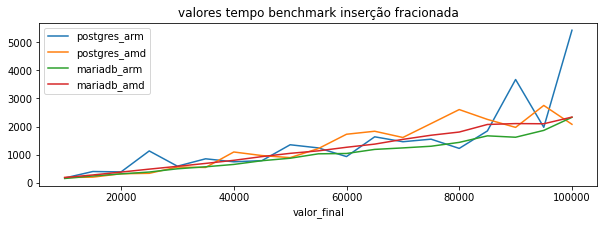
\includegraphics{valores tempo benchmark inserção fracionada.jpg}
  \caption{valores tempo benchmark inserção fracionada}
  \label{fig:resultados insercao fracionada}
\end{figure}


%%%%%%%%%%%%%%%%%%%%%%%%%%%%%%%%%%%%%%%%%%%%%%%%%%%%%%%%
%                      Capítulo 6                      %
%%%%%%%%%%%%%%%%%%%%%%%%%%%%%%%%%%%%%%%%%%%%%%%%%%%%%%%%
 \chapter{Conclusão}
 \label{ch: conclusao}
 


%%%%%%%%%%%%%%%%%%%%%%%%%%%%%%%%%%%%%%%%%%%%%%%%%%%%%%%%
%                      REFERÊNCIAS                     %
%%%%%%%%%%%%%%%%%%%%%%%%%%%%%%%%%%%%%%%%%%%%%%%%%%%%%%%%

% ---
% Finaliza a parte no bookmark do PDF, para que se inicie o bookmark na raiz
% ---
\bookmarksetup{startatroot}% 
% ---

% ---------------------------------------------------------------------------------------------
% ELEMENTOS PÓS-TEXTUAIS
% ---------------------------------------------------------------------------------------------
\postextual


% ---------------------------------------------------------------------------------------------
% Referências bibliográficas
% ---------------------------------------------------------------------------------------------
\bibliography{abntex2-modelo-references}

% ---------------------------------------------------------------------------------------------
% Glossário
% ---------------------------------------------------------------------------------------------
%
% Consulte o manual da classe abntex2 para orientações sobre o glossário.
%
%\glossary

% ---------------------------------------------------------------------------------------------

% Anexos
% ---------------------------------------------------------------------------------------------

% ---
% Inicia os anexos
% ---
\begin{anexosenv}

% Imprime uma página indicando o início dos anexos
\partanexos

\chapter{logs teste de tempo}
%\lstinputlisting[]{apêndices/teste_tempo.log}
\end{anexosenv}

% ---------------------------------------------------------------------------------------------
% INDICE REMISSIVO
% ---------------------------------------------------------------------------------------------

\printindex

\end{document}
